\chapter{Existing technologies}

This chapter describes a classical web application, written in PHP and Javascript, and its conventions helping us design a convenient mechanism of migrating PHP to a browser.
It presents a WebAssembly specification, which follows the existing project using the format to achieve running PHP in a browser.
Give short information about the language CSharp and Mono runtime used in Blazor.
Introduces Blazor and Peachpie, which is integrated by the proposed solution.

\section{PHP and server-side web application}

The basic principle of web pages is a request-response architecture, where a client sends a request for the web page using an HTTP protocol and receives a response with requested data.
A PHP language design makes handling these requests on the server easier.
 
\subsection{Server-side web application}

The previously mentioned principle has several consequences, which are important for our solution.
It is necessary to hold the client's application state on the server because the HTTP is stateless.
An interaction with a page not using next requests is limited by CSS.
HTML presents a tag form as a way how to send additional information to the server after the first request.
The form tag contains other tags representing fields, which are filled by the client. 
Afterward, the form tag enables to encode these data and send it to the server.
Get and post methods are relevant methods, how to perform manner of sending the data.
Get method encodes the data into an URL.
Post method encodes it in the request body, which does not appear in the URL.

\subsection{Language specification}

PHP \cite{5} is interpreted language maintained by The PHP Group.
PHP was designed for generating a web page on the server-side.
Since PHP is a scripting language, its entry-point is the first line of the executing script.

The type system is dynamic.
Variables represent just references to the heap, where all types of objects reside.
An unusual thing is superglobals \cite{6}, which are built-in variables accessible from all scopes of the script.
Following superglobals are relevant to the thesis.
The GET variable stores parsed query part of the URL.
The POST variable stores variables which are sent by post method.
The FILES variable contains uploaded files.
There is also a SESSION variable, which holds a user session.
This variable will become needless because of the proposed solution.

We can divide code in several ways.
Global functions are the most notable characteristic of PHP despite wide-spread object-oriented programming.
They are defined in the global scope and accessible from anywhere.
The next option is an object inspired by object-oriented programming.
There is also namespace support.
And the highest level of division is the module representing the bag of code related to specific behavior like gd2 extension for graphics.

There is not common to use asynchronous functions in a typical PHP application.
One-way pass of the application is a standard convention because of request-response semantic.
The iconic design pattern is Front Controller.
Usually, the main script invokes other parts of the program, based on the request, to deal with it and send the response back.

An HTML interleaving has appeared to be a helpful method for data binding.
The feature allows inserting a PHP code between HTML.
These fragments do not have to form individual independent blocks of code closed in curly brackets. We can see usage of the interleaving in listing \ref{lst:HTMLinterleaving}.

\begin{lstlisting}[basicstyle=\small, caption=HTML interleaving.,
  language=HTML, label={lst:HTMLinterleaving}]
<body>
<h1>Superglobal GET</h1>
<?php
	foreach($_GET as $key => $value) {
?>
	<p><?php echo $key; ?> => <?php echo $value; ?></p>
<?php } ?>
</body>
\end{lstlisting}

Uploaded files sent by the client reside in two places.
The file's information is stored in FILES.
The uploaded file is saved as a temporary file, and standard reading operations can obtain the content.

\section{Javascript and client-side web application}

Control over the rendered page and WebAPI provided by a browser is a point of interest on the client-side.
This functionality usually uses Javascript functions as wrappers. 

\subsection{Client-side web application}

The process of generating a web page follows several steps.
A browser parses the HTML line by line. If a script occurs, the browser starts to execute the code.
The order of processing is important for manipulation with an HTML structure.
This limitation can be solved by web events mentioned later, but
it is a convention to add scripts to the end of the body part after all HTML tags.

We can image a web page as an XML tree.
Its nodes are tags or text fragments, and its edges connect nodes with their children.
One representation of this tree is Document Object Model (abbreviated DOM).
Each node is represented by an object with special parameters relating to HTML and CSS. 
The nodes can contain other nodes representing their children.
Afterward, the document node represents the whole document together with its root node.

Events are the most common method of how to react to changing a web page state.
Every event can have some handlers(listeners).
Whenever an event occurs, it calls all its listeners.
There are many event types, but we will mention the ones that are important for us.
HTML tags are the most common entities, which can have some events.
For example, a button has an event onclick which triggers when a client clicks on the button. 
Other events can represent a state of a page like onload which fires when the whole HTML document is parsed.

A browser provides more APIs valuable for the application, like fetching extra data from a server or local storage.
These APIs are mentioned as Web API \cite{7}.

\subsection{Language specification}

Javascript is a high-level language usually executed by a browser's dedicated Javascript engine but can also be run on a desktop by Node.
It has dynamic typing.
It is often used as a wrapper of Web APIs due to Javascript's essentiality in dynamic web pages.
These APIs are accessible in global scope as an object or global functions.
An example of API available in Javascript can be DOM API mentioned in the previous section.
Javascript supports an event-driven style that helps to react to events conveniently.

Javascript is single-threaded, which can be confusing with its constructs for promises.
Promise is a structure representing an unfinished process.
These processes can be chained.
However, the structure can give an illusion of multi-threading. It uses the scheduler for planning the next task executed by the main thread.
The single thread is critical for blocking operations which causes thread freezing.

\section{WebAssembly}

WebAssembly \cite{9} is a new code format that can be run in today's browsers. 
It has a compact byte format, and its performance is near to a native code. 
WebAssembly is designed to be a compiling target of popular low-level languages like C or C++ due to its memory model. 
It should be able to support languages with carbage collector in the future. 
The advantage of this format is a similarity with Javascript modules ES2015 after compilation into a machine code. 
This enables browsers to execute it by a JavaScript runtime. 
So its security is as good as a code written in Javascript. 
Because of the same runtime, WebAssembly can call Javascript and vice versa.

Threads \cite{10} support is currently discussed nowadays and appears to be realistic.
After all, new versions of Google Chrome experiments with proper multi-threading support despite the chance of vulnerability.
A replacement of multi-threading can be web workers \cite{11}.
The worker's limitation is communication with UI thread only by messages.

Despite supporting to run WebAssembly in a browser, the browser cannot load it as a standard ES2015 module yet.
WebAssembly JavaScript API was created in order to be able to load a WebAssembly to a browser using JavaScript.

\section{Project PHP in browser}

The project \cite{2} aims to use compiled PHP interpreter into WebAssembly, which allows evaluating a PHP code.
The page has to import a specialized module php-wasm. 
A PHP code is evaluated by writing a specialized script block or manually by JavaScript and API.
PHP can afterward interact with JavaScript using a specialized API.
At first glance, that might be a good enough solution, but they are several parts that can be problematic due to PHP semantics.
The solution doesn't solve superglobals. 
This is reasonable because this is the server's job, but you are not able to get information about a query part or handling forms without writing a JavaScript code.
The next problem is navigating how a script can navigate to another script without an additional support code which has to be JavaScript.
These problems can be solved by following technologies and their integration.

\section{CSharp and Mono}

We have to introduce .NET \cite{17} in other to understand the following sections fully.
.NET is a free and open-source project primarily developed by Microsoft.
It is a cross-platform successor to .NET Framework.
It consists of core libraries and runtime, which runs a unique code format CIL standing for Common Intermediate language on various environments.
The runtime is often named CLR (Common Language Runtime) and represents a virtual machine interpreting the code into the machine code.
The libraries can represent whole frameworks like ASP.NET, which aims to web development.
The CIL is a compilation target of languages like CSharp, Visual Basic, or FSharp.
The most common granularity of .NET projects is an assembly formed from a bunch of code representing a library or an executable program.

\subsection{Mono}

Mono is a .NET runtime that aims to mobile platforms. 
Recently, they started to support compilation \cite{12} into WebAssembly.
This support allows executing CIL inside browsers.
The compilation has two modes.
The first one is compilation Mono runtime with all using assemblies.
The second only compile Mono runtime, which then can execute .dll files without further compilation of them into WebAssembly.
A consequence of these compilations into WebAssembly is enabling to call Javascript and WebAPI from .NET.

\subsection{Language specification}

CSharp is a high-level language using strong typing and a garbage collector.
It has a multi-paradigm, but its common characteristic is the objected-oriented style.
These features cause that CSharp is a good language for a huge project which needs discipline from developers to hold the code understandable and manageable.
CSharp is used on the server-side as well as PHP.

\section{Blazor}

Blazor is a framework that provides a convenient way how to write dynamic web pages using CSharp.
Blazor platform is divided into two hosting models \cite{13} which have different approaches to creating web applications. 
The first one is referred to as Blazor Server App and has a similar methodology to a standard website written in PHP.
An interesting innovation is SignalR which is a communication protocol between the server and a client.
However, this thesis uses the second model, which Microsoft refers to as Blazor WebAssembly App enabling offline support after loading the app into a browser.

\subsection{Blazor WebAssembly App}
From now on, I will use Blazor App to refer Blazor WebAssembly App.
Blazor App can be divided into two parts.
The first part serves the main WebAssembly application and its additional resources, which can be requested during runtime.
The second part is WebAssembly wrapped together with an additional user code.
The division enables to choose of a place for the implementation of business logic.
If there is a bad connection, we can move the majority of business logic to the client and use the server for connection to a database; otherwise, we can use the client only for rendering the page. It consists of the following components. 
Kestrel with ASP.NET libraries provides the server part of an application.
Mono runtime compiled to WebAssembly runs CSharp code inside a browser.
WebAssembly is essential for being able to interact with DOM and JavaScript using CSharp without an additional plugin, which was necessary for older technologies like Microsoft Silverlight.
Blazor's libraries provide constructs for manipulation with DOM and WebAPI together with rendering the page and JavaScript interop.
And there is a user's code that using the libraries for creating dynamic pages with CSharp.
A better imagination, how the app is situated on the client-side, can be represented by the figure \ref{img01:wasm} copied from the article \cite{15}.

\begin{figure}[H]\centering
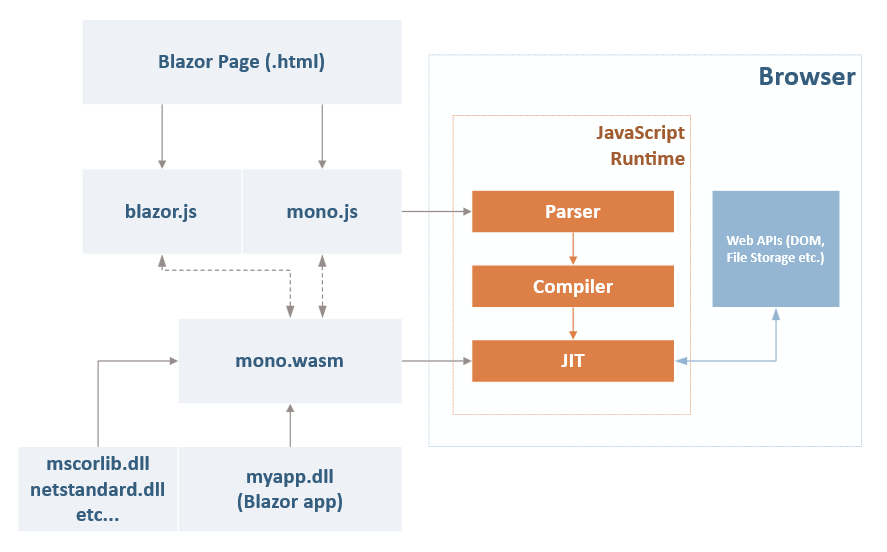
\includegraphics[width=140mm, height=100mm]{./img/BlazorExecution}
\caption{Running a Blazor WebAssembly App on client-side.}
\label{img01:wasm}
\end{figure}

The interop with a browser are one part of the Blazor App.
The main part is the architecture of the libraries.
A common approach how to create a page is using the markup language Razor.
There already exists Razor in standard ASP.NET website where .cshtml extensions consist of this markup.
Unfortunately, the markup used in BlazorApp has the same name.
From now on, I will use Razor for the markup language, which is the content of .razor files in Blazor App.
Because interleaving HTML with other languages turns out to be helpful, the Razor uses special characters to identify CSharp code in HTML and convert it to rich content pages.
A significant purpose of Razor is for generating CSharp structures, which represent parts of a page, during compilation time.
These structures have a complex interface for rendering a page, so the markup is there in order to free users using a complicated mechanism for putting a page together. 
We can see an example of web page in listing \ref{lst:razorpage}.

\begin{lstlisting}[basicstyle=\small, caption=Example of Razor page., label={lst:razorpage}]
@page "/example"
@inject HttpClient Http

<h1>Example</h1>
@if (!loaded)
{
    <p>Loading...</p>
}
else
{
    <p>Ticks: @ticks</p>
}

@code {
    private bool loaded = false;
    private int ticks = 0;

    protected override async Task OnInitializedAsync() {
        ticks = await Http.GetFromJsonAsync<int>("ticks.json");
        loaded = true;
    }
}
\end{lstlisting}

Razor provides a special sign at which follows with dedicated keywords.
We can see a page keyword determining the path of the page. An inject keyword represents a service injection. An if keyword determines a standard condition, and a code keyword contains a regular CSharp code.
These features are afterward transformed into CSharp entities forming a special class.

Blazor introduces a Component class that can represent a whole page or the part of it.
Components can be arbitrarily put together in order to form the desired page.
We can see the generated Component from listing \ref{lst:razorpage} in listing \ref{lst:component}.

\begin{lstlisting}[basicstyle=\small, caption=Razor page generated to the CSharp class., label={lst:component}]
[Route("/example")]
public class Index : ComponentBase {
	private bool loaded = false;
	private int ticks = 0;
	
	[Inject] private HttpClient Http { get; set; }

	protected override void BuildRenderTree(RenderTreeBuilder __builder) {
		__builder.AddMarkupContent(0, "<h1>Example</h1>");
		if (!loaded)
		{
			__builder.AddMarkupContent(1, "<p>Loading...</p>");
			return;
		}
		__builder.OpenElement(2, "p");
		__builder.AddContent(3, "Ticks: ");
		__builder.AddContent(4, ticks);
		__builder.CloseElement();
	}

	protected override async Task OnInitializedAsync() {
		ticks = await Http.GetFromJsonAsync<int>("ticks.json");
		loaded = true;
	}
}
\end{lstlisting}

We can assign the Razor keywords to parts of the code in the listing.
Page keyword stands for Route attribute.
Inject keyword stands for parameter attribute. The parameter is assigned by a dispatcher, mentioned later, during the initialization.
Code keyword is a part of class content.
Another markup is transformed into calling a specialized method in the BuildRenderTree function, which renders the page. 
There will be more information about rendering later in this section.

The components can have different purposes. For example, a Router takes care of routing the right page whenever the navigation is triggered.
Alongside components, a dispatcher supplies additional services like logger to components when they are creating.
The dispather is a specialized class initialized in the begining of the application.

The last item, which is not used transparently, is a WebAssemblyHost builder.
The builder configures the application and prepares the renderer used by components to render their content.

Balzor presents its own virtual DOM to reduce changing a DOM directly in a browser to its demanding performance.
A component works with RenderTreeBuilder, which provides an interface for adding content to the virtual DOM.
The usage of RenderTreeBuilder is complex due to Blazor's diff algorithm, which is used afterward.
RenderTreeBuilder is just a superstructure over Renderer, which is responsible for updating the page.
The diff algorithm is used to minimize the browser's DOM  update after all components used RenderTreeBuilder to render their content.
This algorithm used sequence numbers for parts of HTML to identify modified sections.
Sequence numbers respond to an order of RenderTreeBuilder's instructions in the source code.
A benefit of this information is detecting loops and conditional statements to generating smaller updates of DOM.  
It follows the browser's DOM update, which is executed by Blazor's JavaScript support code called through Mono runtime.

The process of bootstrapping the Blazor App to a browser follows these steps. 
Kestrel gets a request for a page that is contained in Blazor App. 
The server responses with the index.html page, which contains references to JavaScript support code (This code is referred to as blazor.js and mono.js in the figure \ref{img01:wasm}) responsible for loading and running the runtime with the application part.
The runtime runs the application using the Main method in Blazor App.
The remaining interactions are maintained by event handling.
I distinguish two types of events.
The first type is navigation.
The navigation \cite{14} can be triggered by an anchor, form, or filling up the URL bar.
The URL bar is handled separated by a browser.
JavaScript can influence the remainings elements.
Blazor App handles only an anchor by.
After clicking on an anchor, predefined methods in blazor.js try to invoke navigation handler in Blazor App using a Mono WebAssembly gateway.
A user can modify this handler, but a specialized component Router implements a default behavior.
The Router finds out all components, which implements an IComponent interface, by a reflection and tries to render the page according to path matching RouteAttribute of a component.
The navigation can be redirected to the server if there is no match.
The second type is events invoked by UI like onchange. These event's callbacks call right CSharp callbacks thanks to RenderTreeBuilder, connecting CSharp callback with element's event.

\section{Peachpie}

Peachpie \cite{16} is a modern compiler based on Roslyn and Phalanger project.
It allows compiling PHP into a .NET assembly, which can be executed alongside standard .NET libraries.
Peachpie introduces several structures representing states, scripts, and variables of PHP written in Csharp.
The first of them is a context representing one request to PHP code.
The context consists of superglobals, global variables, declared functions, declared and included scripts.
The possibility of saving the context and using it later is a significant advantage used in the solution.
The context can also be considered as a configuration of the incoming script's execution.
All information about a request can be arranged to mock every situation on the server-side.
The compiler offers a dedicated type of assembly for PHP libraries.
Using this assembly can add additional functions, which can provide an extra nonstandard functionality as an interaction with a browser.
Another advantage of the compiler is the great interoperability between PHP and .NET.
An option to work with Csharp objects, attributes and calling methods will become crucial for achieving advanced interaction between Blazor and PHP.

However, there are limitations following from differences in the languages and the stage of development.
Availability of PHP extensions depends on binding these functions to CSharp code which gives equivalent results. The time and memory complexity of this code can be tricky in Blazor.
The previously mentioned interoperability has limits as well.
Csharp constructs like structs and asynchronous methods are undefined in PHP.


